
%===========================================
\section{App Development Process}
%===========================================
This chapter summarizes important steps concerning the development process of our app.
We do not provide in-depth insight to our implementation. 
Instead we give a brief overview of our approach for the development of a user friendly and understandable app.
%===========================================
\subsection{Mock Up}
\label{s:mockup}
%===========================================
After we decided about the work flow and structure of our app we built a mock up in order to get a more concrete idea of what needs to be implemented and to reveal flaws in our thought process.
We showed it to friends and relatives so we could expose aspects we have not yet thought about.
The first texts explaining how to access the address bar and the structure of a URL seemed to be difficult to understand.
As a consequence, we adjusted these texts in the app (only those of the first three levels) and showed them to other friends and relatives who seemed to understand the descriptions.
Based on these initial texts we wrote all remaining texts without including it into the app yet.
The next section describes the elaboration process of these texts.
%===========================================
\subsection{Pilot Study of App Texts}
\label{s:pilot_study}
%===========================================
After finishing the texts for each step of the app flow (the texts were not directly included into the app) our supervisor, a professor of pedagogy at TU Darmstadt as well as another highschool teacher of German reviewed them.
Once we achieved the version with which we were satisfied we applied a user study on it. 
For time reasons, we decided to go for the low cost method of guerilla user testing~\cite{guerillagovuk, guerillauxbooth}.
This approach enables to quickly assess the effectivity of a design, in our case our app texts.
Guerilla user tests is rather loosely structured and do not include participant recruitment.
The testers are rather approached, in our case, we asked relatives and friends. 
The outcome of such studies is rather qualitative, i.e. extensive and detailed insights are achieved.
A downside of guerilla testing is that the approached participants might not belong to the defined target group with respect to their expertise or skills. 
Since we knew our participants we addressed only those who matched our target audience. 
In detail, our approach for the guerilla user test was as follows:

\begin{enumerate}
	\item\textit{Preparation of Texts:} Our aim for this user test was to imitate the use of a smartphone as best as possible.
	For this reason, the app texts were formatted into short lines, so that the text appearance resembled that of a smartphone screen.
	Furthermore, we printed out the texts and cut the sheets into small rectangles.
	\item\textit{Think Aloud:} We asked the participants to think aloud during the test. 
	We told them that there are no stupid questions or comments and that they help most with just saying what goes through their mind.
	We made notes of their remarks.
	\item\textit{User Test with In-Between Exercises:} The actual user test mainly consisted of reading our app texts and thinking aloud about these.
	We included a little simulation of our exercise parts in order to validate whether the users comprehended the texts or not.
	For example, for each introduced attack we included a small list of URLs on which the users had to decide whether they were phishing URLs or not.
	\item\textit{Final Comments:} After going through the texts the users were asked to provide their general impression.
	We further asked them about some aspects we were not quite sure about at the beginning. 
	For example, we asked them whether the usage of the terms ``link'' or ``web address'' confused them, which was not the case.
\end{enumerate}
Our guerilla user tests showed that our texts are understandable.
According to our participants the main downside of the texts was their length. 
Yet, this can be neglected since the users had to read our complete texts (instead of for example just playing 1-2 levels at once). 
Furthermore, they remarked that the introduction on how to access the whole address bar and analyze the complete URL is unnecessary. 
For some users this might apply. 
However, it is possible that there are users who do not know this. 
For those who already know how to access the address bar and analyze the complete URL we added a button which directly links to the exercise. 
In case the user had overestimated himself, he will be forwarded back to the app, where the introductory text can be consulted. 
Finally, the provided brief summary of already passed lessons (reminder texts) received some criticism for their frequent re-appearance at the beginning of each level. 
This can also be neglected since we assume that our app users will not constantly play this game and in our view repetitive serving of the major lessons learned is helpful to internalize them (cf. Principle of Exercise in \autoref{s:learning_principles}). 
Also, when playing the app this screen can easily be skipped as it exhibits a recognition value achieved by the title ``reminder''. 
Moreover, we decided for a minor reorganization of the reminder view. 
Before the user tests the reminders mainly referred to the URL structuring they have learned so far. 
We thought it is also important to remind the users of possible attacks. 
Therefore, the reminder concerning the URL structure was kept to a minimum with the aid of a graphic. 
Plus, for each attack in previous levels one sentence and one example was added.  
To sum it up, the introductory blocks that introduce spoofing techniques of phishers (level 2-9) are generally structured as follows:
First, we provide the major lessons learned from the previous levels in the reminder.
An example reminder view of level 3 is depicted in  cf. \autoref{fig:Screenshot_intro2}.
Next, a brief introduction to the current level's topic follows.
Finally, the new attack is introduced which includes one or more examples.
An example of this view is shown in \autoref{fig:Screenshot_intro3}.

\begin{figure}[hHtbp]
\centering
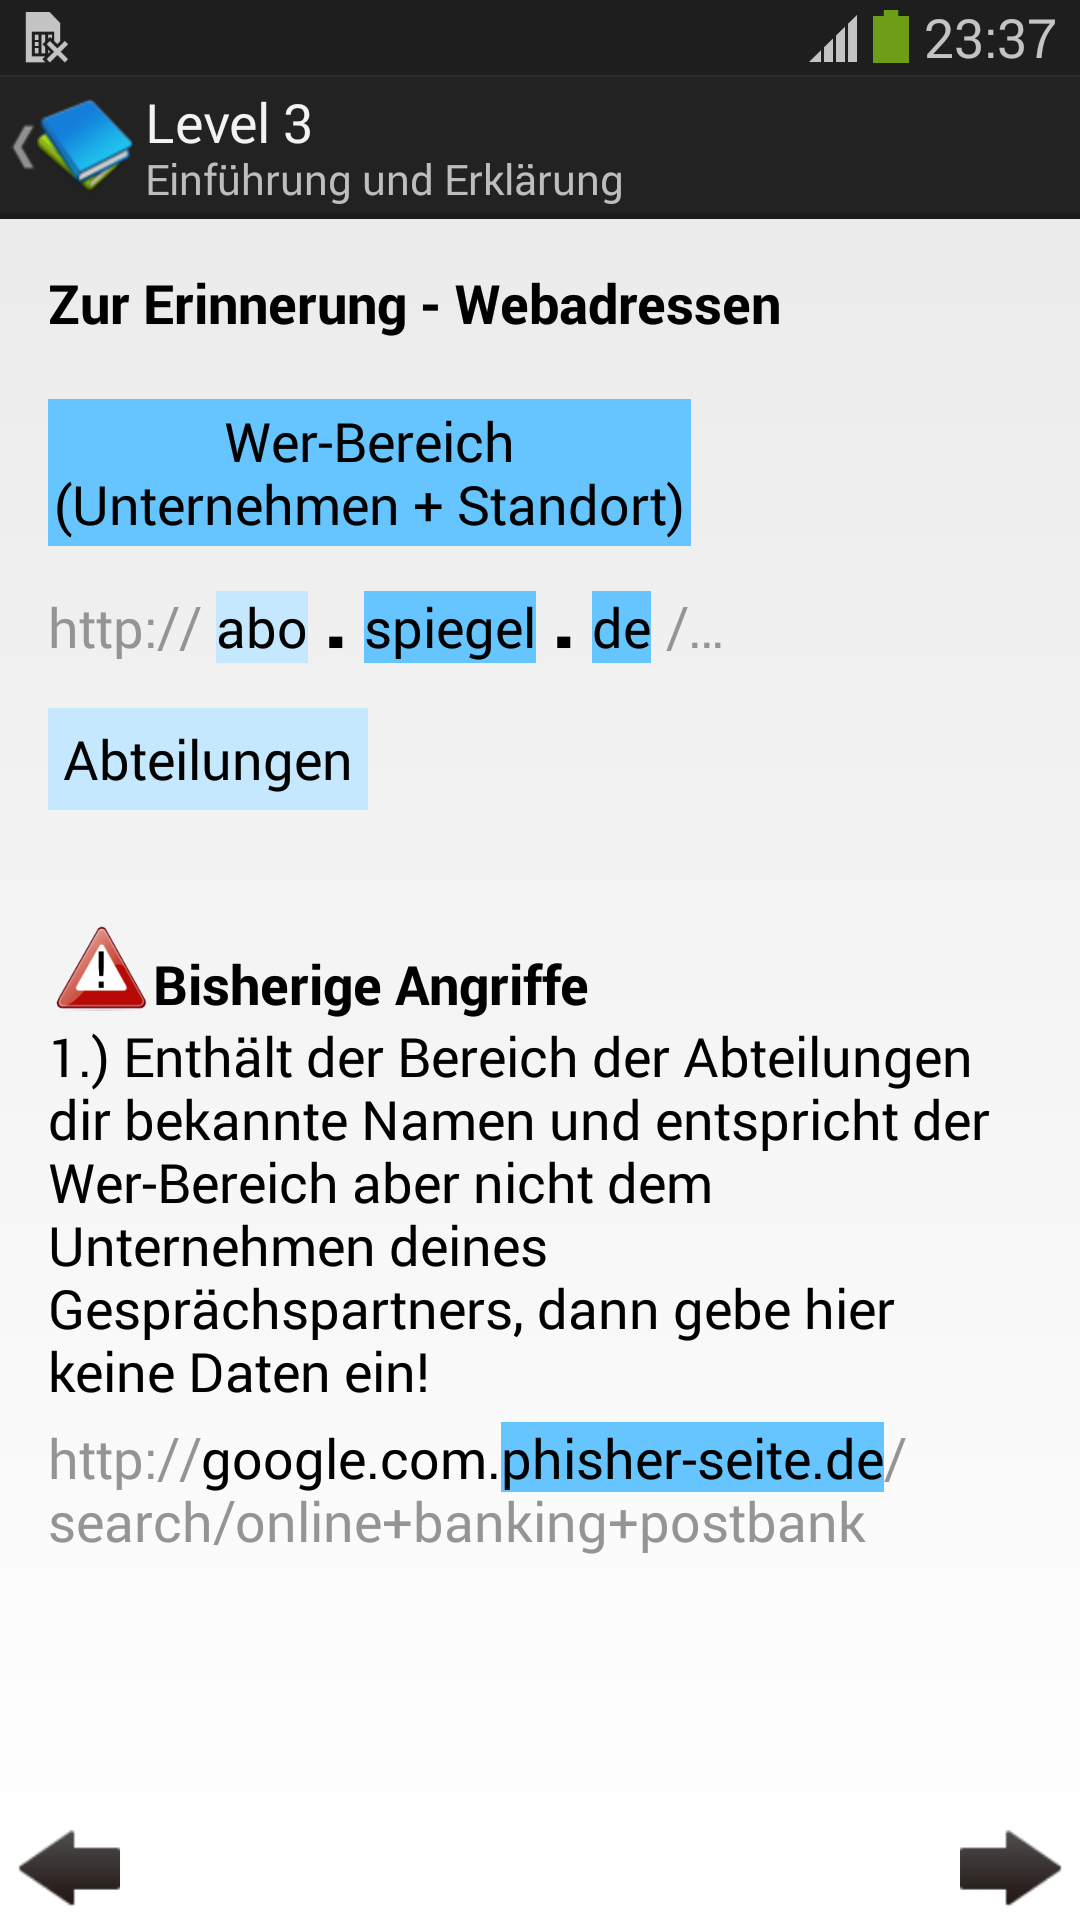
\includegraphics[width=0.4\textwidth]{Screenshot_intro2.png}
\caption{Example reminder view of level 3}
\label{fig:Screenshot_intro2}
\end{figure}


\begin{figure}[hHtbp]
\centering
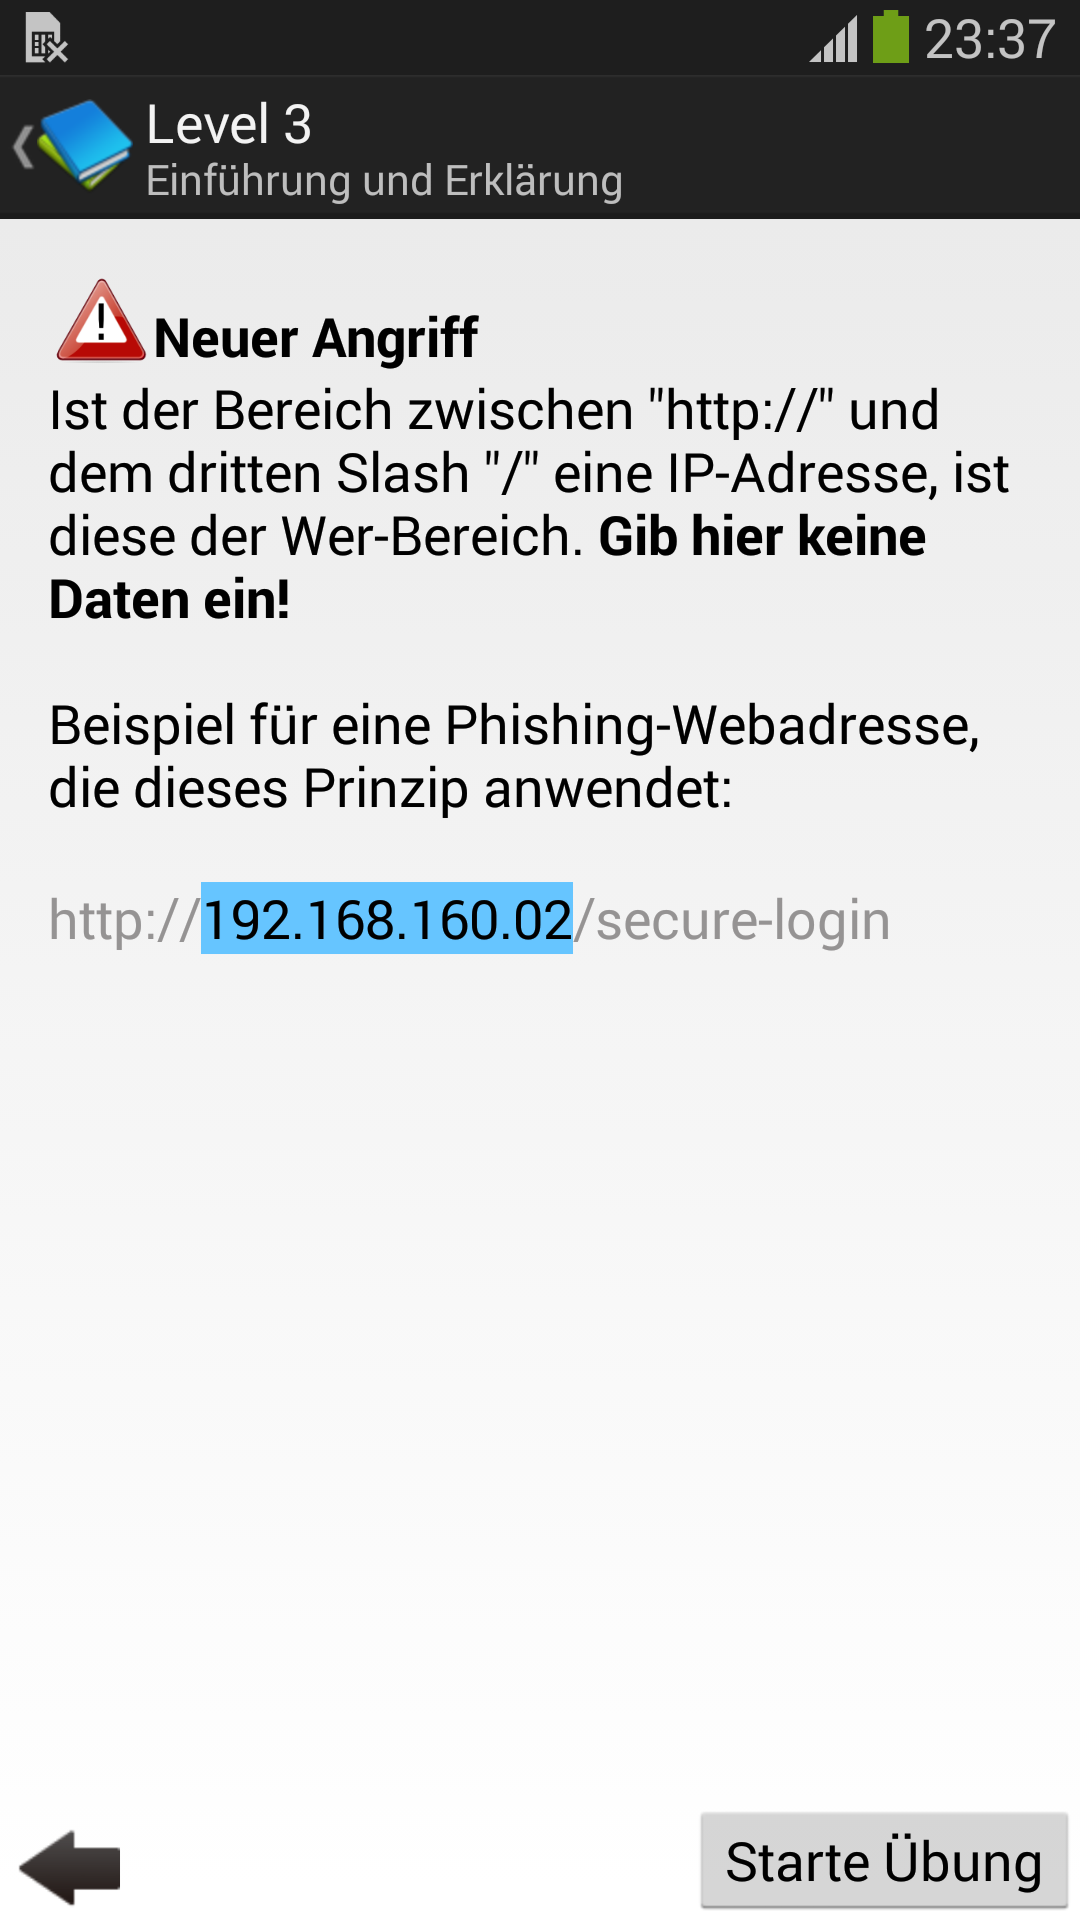
\includegraphics[width=0.4\textwidth]{Screenshot_intro3.png}
\caption{Example view of new attack in level 3}
\label{fig:Screenshot_intro3}
\end{figure}


%--------------------------------------------------------
\subsection{Legibility Index of Our Texts}
\label{s:legibility_index}
%--------------------------------------------------------
Comprehensibility is of major importance for our app. Each level starts with a lesson on a certain way phishers make use of in order to delude people. These lessons aim to educate the user by describing those phishing attempts. Hence, it is of utter importance that our explanations are both thorough as well as comprehensible. After we had conducted user tests and included their corresponding valuable feedback (cf.\autoref{s:pilot_study}) and also received good feedback from the final study (cf.~\autoref{s:further_exploration}), we now want to assess the comprehensibility of our texts with the aid of a statistical method. Several approaches to assess the readability of a given text exist~\cite{Gun,citeulike:7369187}. These approaches consider, among other details, the average word and sentence length and therefore are language dependent and usually are designed for the English language. However, the Flesch-Reading-Ease~\cite{citeulike:7369187} is a legibility metric that outputs a numeric indication for the readability of the input text and was also adjusted to operate with the German language by Toni Amstad~\cite{amstad1978verstandlich}. The readability of a German text is computed as follows, where $\operatorname{ASL}$ represents the average sentence length and $\operatorname{ASW}$ the average number of syllables per word:
$$\operatorname{FRE_{German}} = 180-\operatorname{ASL}-(58.5\times\operatorname{ASW})$$
Several auxiliary tools exist that take a regular text as their input and return a legibility index as their output~\cite{leichtlesbar, stilversprechend,fleschindexde}. All of these tools delivered different scores because they obviously had varying algorithms to determine syllables, sentences and even word boundaries.
Therefore, we approached as follows: First, we took the explanation part of each level as the input for all of the three tools. Second, we extracted the amount of sentences, words, and syllables from the returned values, as depicted in~\autoref{table:legibillity_index}. We did not rely on the returned legibility indexes, because the tools seemed to use slightly different formulas. Third, with the extracted information we were able to compute the German FRE index ourselves in a consistent way through all of the three tools. Ultimately, we derived a final index value of 62 by averaging the resulting index values of each tool. Given a scale from 0 to 100, where an index of up to 30 indicates an academic level and 90 and above is considered easy to understand, an index of 62 is considered as reasonably comprehensive for teenagers~\cite{amstad1978verstandlich}. Regarding our target group, this is a good result and confirms the comprehensibility of our explanations also statistically.

\begin{table}[hHtbp]
\centering

    \begin{tabular}{|llll|}
    \hline
     &\textbf{Leichtlesbar.ch} &\textbf{Stilversprechend.de} &\textbf{Fleschindex.de}\\ \hline
    \textbf{\# Sentences}		& 426	& 604	& 400\\
    \textbf{\# Words}			& 4616	& 4760	& 4762\\
    \textbf{\# Syllables} 		& 8305	& 8658	& 9235\\
    \textbf{Legibility Index}	& 64	& 66	& 55\\
    \hline
    \end{tabular}
    \caption{Sentences, words and syllables of our texts outputted by different tools~\cite{leichtlesbar, stilversprechend,fleschindexde}}
    \label{table:legibillity_index}
    
\end{table}



\subsection{Implementation and Testing}
\label{s:implementation_testing}
In parallel to formulating and validating our app texts we developed the basic structure and logic of our app.
After conducting and assessing the guerilla user tests of our texts and integrating the feedback, we started to include them into our app.
We both developed and tested the app simultanously.
Occasionally, we showed the app to friends and relatives in order to get some feedback on aspects we might have missed.
In this way, our app was formed incrementally. 
We do not intend to provide implementation details in this work.
The only exception is the algorithm used to generate the URLs on which the users have to decide whether they are phishing URLs or not. This approach can be consulted in \autoref{s:url_generation}.
